\documentclass{article}[18pt]
\usepackage{../../../../format}
\lhead{Software Engineering - Modelling and Analysis}


\begin{document}
\begin{center}
\underline{\huge Modelling Objects}
\end{center}
\section{Characteristics of Objects}
Objects have a distinct set of characteristics, not all of which readily lend themselves to modelling\\
\\
Some key characteristics are:
\begin{itemize}
	\item They are uniquely identifiable runtime entities
	\item Objects can be composed, that is, the object's data variables may themselves be objects
	\item The implementation of an object can be reused and extended through inheritance, to define other objects
	\item OO code can be polymorphic, using generic code that will work with related but different types
\end{itemize}
Inheritance and polymorphism are both difficult to include in a diagrammatic model
\section{The UML}
The Unified Modelling Language (UML) is now more or less the de facto standard for describing object oriented systems\\
\\
Essentially it draws together (unifies) three earlier modelling forms, and does not do it particularly well. Empirical evidence suggests that is is not very widely used for developing models, although sometimes it is used for formalising them.\\
\\
However, it has extensive documentation and tool support, so hard to avoid using it in some form\\
\\
The practices of "design methods" developed in the "structured design" era tend to begin with the creation of single-viewpoint models, For example:
\begin{itemize}
	\item Start with a functional model using DFDs
	\item Elaborate this into greater detail
	\item Possibly augment with STDs
	\item Transform the DFDs into Structure Charts to produce a constructional model
\end{itemize}
In contrast, OO methods tend to begin by identifying "real-world" objects and all their interactions. So from the start, the design model needs to describe many characteristics, based upon several viewpoints\\
\\
A major criticism of the UML is that the outcome is a set of notations that are:
\begin{itemize}
	\item Overly complex and unwieldy
	\item Lack any overarching "viewpoints" concept, making it hard to integrate them in any sense
	\item There is also some overlap between many of the notations (diagram forms) because of the diverse set of forms used in the earlier OO modelling that were merged into the UML
\end{itemize}
\section{Statecharts}
The Statechart has a mathematical underpinning. Claimed to result in a model that is relatively unambiguous and less dependent upon text to provide semantic interpretation than most diagrammatic forms\\
\\
The notation supports:
\begin{itemize}
	\item Clustering of states to form super-states
	\item Orthogonality of states
	\item Stepwise refinement of states
\end{itemize}
Much of this is now incorporated in the UML
\subsection{Hierarchy in statecharts}
\begin{center}
	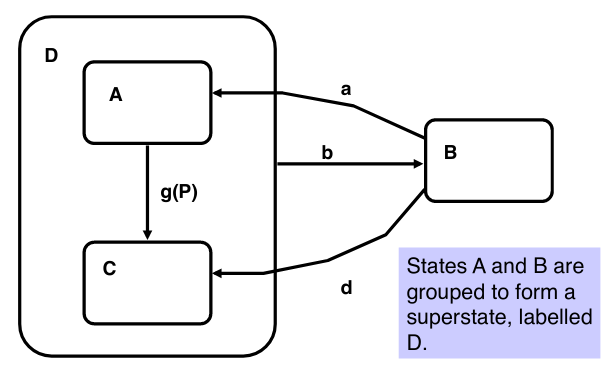
\includegraphics[scale=0.7]{statecharts}
\end{center}
\section{The Sequence Diagram}
\begin{defin}[Sequence Diagram]
	A diagram that shows object interactions arranged in time sequence. In particular, it shows the objects participating in an interaction and the sequence of messages exchanged
\end{defin}
A sequence diagram visually describes a pattern of interaction arranged in time order\\
\\
The sequence diagram describes the system from a functional viewpoint: it is largely concerned with how interaction amongst objects is organised
\subsection{Variations}
The sequence diagram can have two roles:
\begin{itemize}
	\item Descriptor form - mostly used for the purposes of systems analysis and tries to describe all possible scenarios for object interaction
	\item Instance form - Mostly used in requirements modelling and design, where we might want to model the specific object interactions that occur in one actual scenario
\end{itemize}
\subsection{Notation}
\begin{itemize}
	\item The vertical dimension is used to indicate time, generally proceeding down the page
	\item The horizontal dimension represents each of the objects that are to take part in a pattern of interaction: each object is shown in a separate column
	\item An object symbol (a rectangular text-box) appears in its column at the point in time that the object is created. The object's lifeline descends from it and is a dashed line if the object is acquiescing or a long thin rectangle if it has an active focus of control
	\item Messages between objects are shown as solid horizontal arrows between the lifelines of the sender and recipient
\end{itemize}
\begin{center}
	\includegraphics[scale=0.7]{"sequence diagram"}
\end{center}
\subsection{Additional features}
Sequence diagrams can have lots of optional features including:
\begin{itemize}
	\item Timing constraints
	\item Distinguishing between asynchronous control and procedural control
	\item Showing deletion of objects
\end{itemize}
The advice is to keep it simple and use the instance form for any initial modelling sketches
\section{The class diagram}
Can be used to model objects that do things and also data objects. (here it acts as an entity-relationship diagram, although empirical studies show that it provides a poorer visualisation than an ERD)\\
\\
Different levels of detail in the formalisation (can add information about methods, data etc in the boxes)\\
\\
This notation is widely used, including by many tools
\begin{center}
	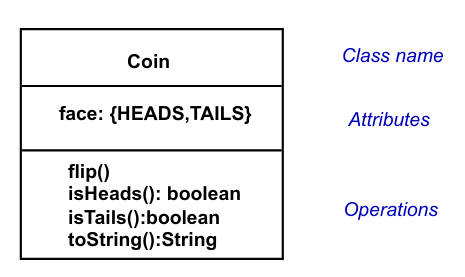
\includegraphics[scale=0.7]{class}
\end{center}
Converted to UML it would look like this
\begin{center}
	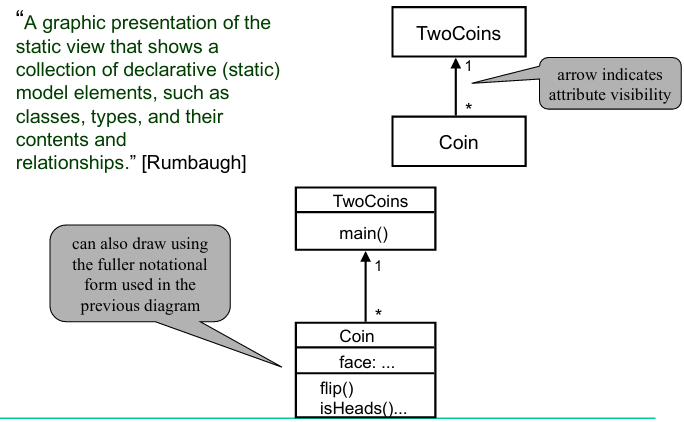
\includegraphics[scale=0.7]{class-uml}
\end{center}
The arrow heads mean as follows
\begin{center}
	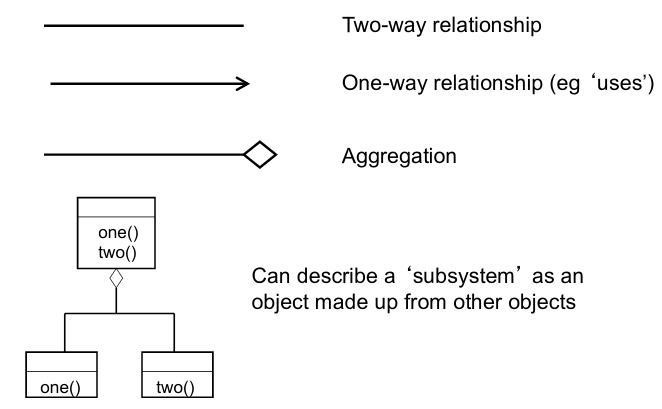
\includegraphics[scale=0.7]{arrows}
\end{center}
\section{Analysis}
The abstract nature of diagrammatic models makes it difficult to conduct formal and rigorous analysis\\
\\
Models typically address ideas about:
\begin{itemize}
	\item Information
	\item Behaviour
	\item Architecture
	\item Application domain
	\item Business/enterprise
\end{itemize}
Analysis usually addresses such characteristics as:
\begin{itemize}
	\item Completeness and consistency
	\item Correctness
	\item Dependability
\end{itemize}
\subsection{How do we a analyse such models?}
Various techniques, just mention two here
\begin{itemize}
	\item Tabulation for cross checking (completeness)
	\begin{itemize}
		\item A bit like the earlier example of an STT. If we tabulate different relationships, we can check our model for any omissions, or inconsistencies. A simple but often quite effective method
	\end{itemize}
	\item Use of walkthroughs and scenarios (correctness)
	\begin{itemize}
		\item Usually a team thing, involving walking through a model working out how it will behave in response to various stimuli and under specific conditions
		\item The basis is usually one or more scenarios of use
	\end{itemize}
\end{itemize}




\end{document}